%
% $Id: cruise_listbox.tex,v 1.2 2002/02/12 22:15:32 wolli Exp $
%
\section{Kommando 'listbox'}
\kw{listbox} \am{Liste Feldreferenz}

\subsection{look and feel}
Das Bild zeigt die Listbox w�hrend der Interaktion.

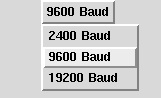
\includegraphics{cruise_listbox.eps}
\subsection{Verhalten w�hrend Interpretation}
Erzeugt eine Box mit dem Inhalt, welcher durch \am{Feldreferenz} referenziert wird.

\subsection{Verhalten bei Interaktion}
Wird die Box mit dem aktuellen Inhalt angeklickt, so �ffnet sich eine Auswahlliste
mit den Eintr�gen wie sie in \am{Liste} angegeben wurden. Der Benutzer kann
nun durch Auswahl eines Listeneintrags den neuen Wert bestimmen. Die
Auswahlliste verschwindet und an die durch \am{Feldreferenz} angegebene 
Stelle wird der ausgew�hlte Wert geschrieben.

\subsection{Beispiel}

\verb*|listbox {"2400 Baud" "9600 Baud" "19200 Baud"} l:p1 c:3|

erzeugt bei Interaktion eine Auswahlliste wie oben dargestellt.
